\newpage

\section{평가}
\label{sec:evaluation}
\begin{figure}[h!]
  \begin{center}
    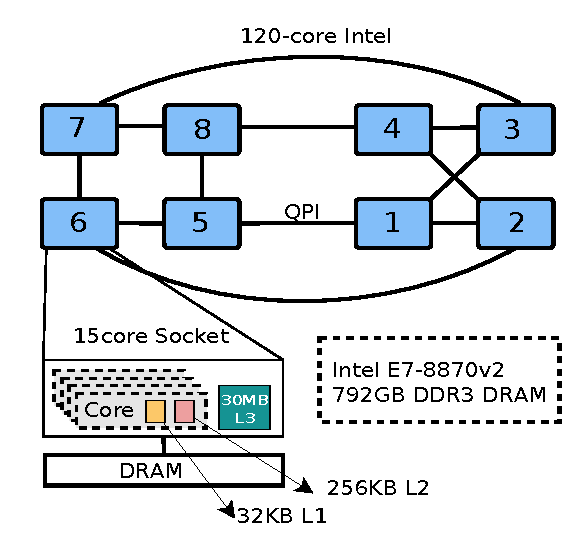
\includegraphics[scale=0.8]{fig/xeon}
  \end{center}
  \caption{실험 환경.}
  \label{fig:xeon}
\end{figure}
 
 \begin{figure}[h]
    \centering
    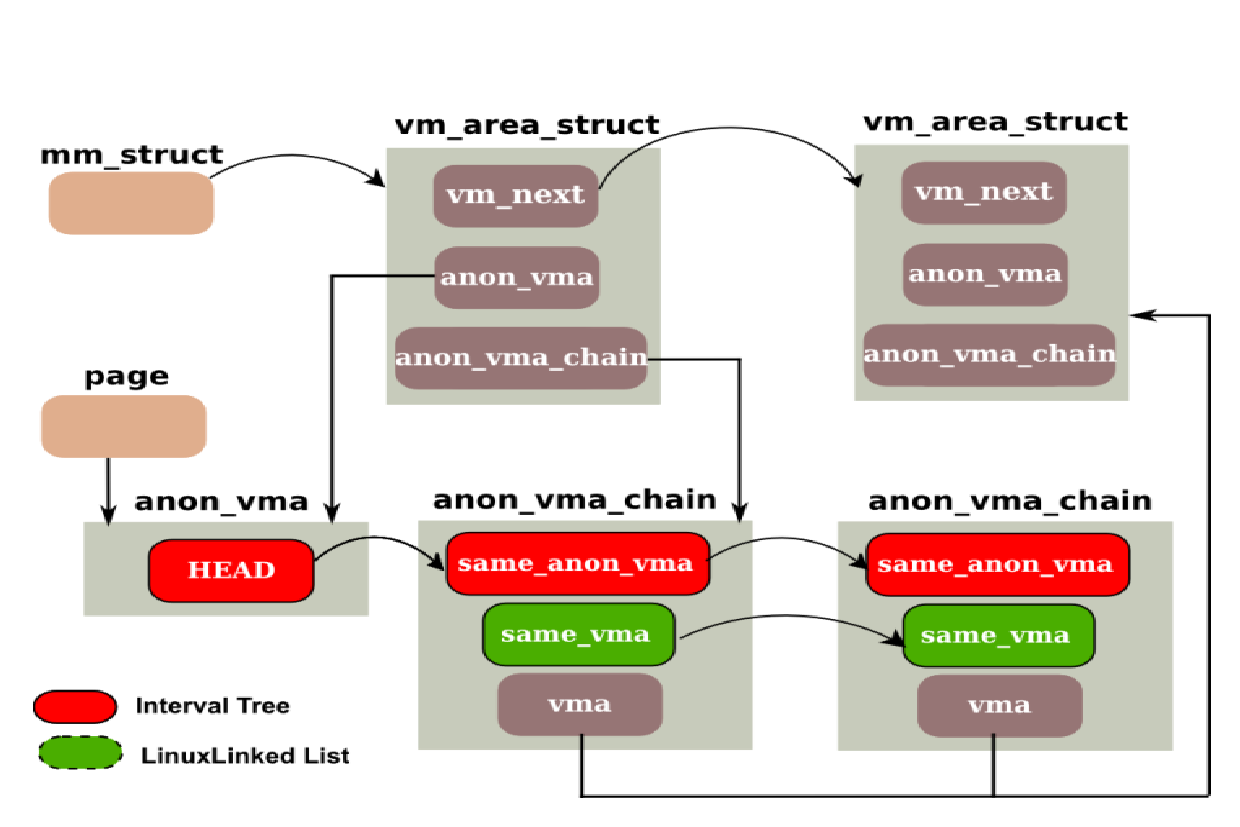
\includegraphics[width=0.8\textwidth]{fig/lockfree}
    \caption{Harris 리스트로 변경하기 전 자료구조}
  \label{fig:lockfree}
\end{figure}
 
 \begin{figure}[h]
    \centering
    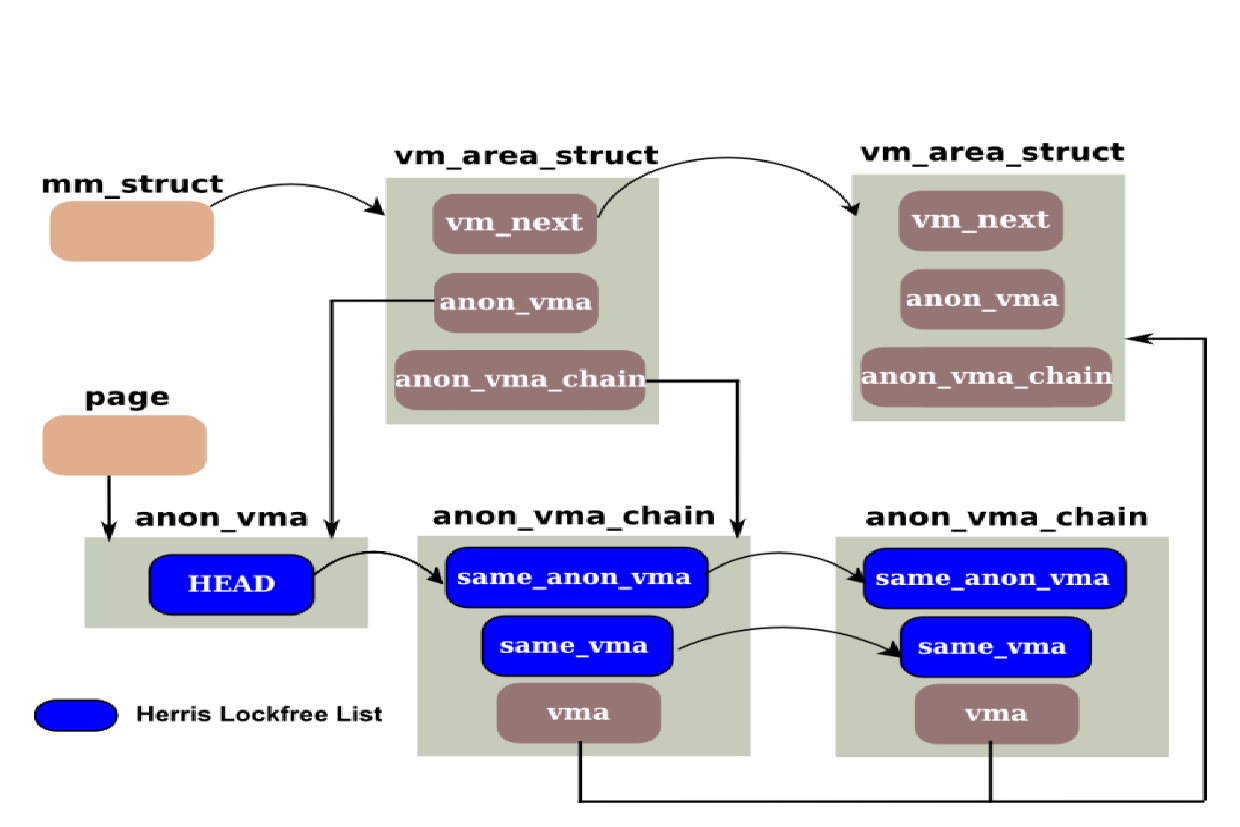
\includegraphics[width=0.8\textwidth]{fig/lockfree_2}
    \caption{Harris 리스트로 변경 후 자료구조}
  \label{fig:lockfree_2}
\end{figure}

\subsection{실험 환경}

%$$$$$$$$$$$$$$$$$$$$$$$$$$$$$$$$$$$$$$$$$$$$$$$$$$$$$$$$$$$$$$$$$$$$$$$$$$$$$$$$
%Paragraph 3: 운영체제 및 커널 버전 설명
%$$$$$$$$$$$$$$$$$$$$$$$$$$$$$$$$$$$$$$$$$$$$$$$$$$$$$$$$$$$$$$$$$$$$$$$$$$$$$$$$
실험을 위해 사용한 하드웨어는 8소켓으로 구성된 120코어 시스템을 사용했으며,
각각의 코어는 인텔 E7-8870 chips(소켓당 15 코어)을 가진다.
메모리는 792기가 바이트 DDR3 DRAM을 사용하였다.
그림~\ref{fig:xeon}은 우리가 사용한 시스템을 보여준다.

%$$$$$$$$$$$$$$$$$$$$$$$$$$$$$$$$$$$$$$$$$$$$$$$$$$$$$$$$$$$$$$$$$$$$$$$$$$$$$$$$
%Paragraph 1: 무엇을 평가 했는지에 대한 설명 
%$$$$$$$$$$$$$$$$$$$$$$$$$$$$$$$$$$$$$$$$$$$$$$$$$$$$$$$$$$$$$$$$$$$$$$$$$$$$$$$$
본 논문에서 제안한 LDU 기법에 대해 평가를 하기 위해, 우리는 리눅스 커널에 LDU를 적용하여 성능을 비교하였다.
비교 대상으로는 수정하지 않은 리눅스 커널과 Harris의 \code{lock-free} 리스트~\cite{Harris2001Lockfree}
알고리즘을 리눅스 커널에 구현하여 추가로 비교 실험을 하였다.
Harris 알고리즘을 사용한 이유는 논블락킹 알고리즘 중에서 대표적인 알고리즘이기 때문이다. 
Harris의 링크드 리스트의 알고리즘은
\textit{sysnchrobench}~\cite{Gramoli2015Synchrobench}와
\textit{ASCYLIB}~\cite{David2015ASYNCHRONIZED}에서 구현된 내용을 이용했으며, Harris 링크드 
리스트를 리눅스 커널에 맞게 수정하여 적용하였다.
Harris 링크드 리스트에 대한 적용을 예를 설명하면, 기존 리눅스는 그림~\ref{fig:lockfree}과 같이 
\code{anon\_vma\_chain}의 내부 변수 중 \code{same\_anon\_vma}는 인터벌 트리로 되어 있고, 
\code{same\_vma}는 리눅스의 링크드 리스트로 되어 있다. 
두 자료구조를 그림~\ref{fig:lockfree_2}와 같이, 
논블락킹 링크드 리스트 중 하나인 Harris 링크드 리스트로 수정하여 구현을 하였다.


%$$$$$$$$$$$$$$$$$$$$$$$$$$$$$$$$$$$$$$$$$$$$$$$$$$$$$$$$$$$$$$$$$$$$$$$$$$$$$$$$
%Paragraph 2-1: Harris Lock free list 구현 내용에 대한 설명 
%$$$$$$$$$$$$$$$$$$$$$$$$$$$$$$$$$$$$$$$$$$$$$$$$$$$$$$$$$$$$$$$$$$$$$$$$$$$$$$$$

%$$$$$$$$$$$$$$$$$$$$$$$$$$$$$$$$$$$$$$$$$$$$$$$$$$$$$$$$$$$$$$$$$$$$$$$$$$$$$$$$
%Paragraph 1: 벤치 마크 대한 설명
%$$$$$$$$$$$$$$$$$$$$$$$$$$$$$$$$$$$$$$$$$$$$$$$$$$$$$$$$$$$$$$$$$$$$$$$$$$$$$$$$
본 연구에서 개발한 LDU는 \code{fork}에 집약적인 응용프로그램과 업데이트 비율이 높은 
자료구조가 효율적인 알고리즘이다. 
따라서, \code{fork}에 집약적인 벤치마크를 선택하였다. 
본 연구에서 선택한 벤치마크 프로그램들은 리눅스의 확장성 벤치마크인 AIM7, 그리고 MOSBENCH에서 
구현된 이메일 서버 벤치마크인 Exim 그리고 마이크로 벤치마크인 Lmbench 이다.
이러한 워크로드들은 모두 역 매핑 때문에 높은 락 경합을 보여준다. 
먼저 AIM7 벤치마크는 리눅스 커뮤니티에서 리눅스 커널에 대한 테스팅 뿐만 아니라 
확장성을 향상 시키기 위해 많이 사용되는 벤치마크이다.
Exim은 실제 사용되고 있는 오픈 소스 응용프로그램이다. 
하지만 이것 역시 리눅스 \code{fork} 때문에 성능에 대한 병목 현상이 발생한다.
마지막으로 마이크로 벤치마크 형식의 \code{fork}에 대한 성능과 확장성에 대해서 보기 위해 
Lmbench를 선택하였다. 

%$$$$$$$$$$$$$$$$$$$$$$$$$$$$$$$$$$$$$$$$$$$$$$$$$$$$$$$$$$$$$$$$$$$$$$$$$$$$$$$$
%Paragraph 2: 비교 대상에 대한 설명
%$$$$$$$$$$$$$$$$$$$$$$$$$$$$$$$$$$$$$$$$$$$$$$$$$$$$$$$$$$$$$$$$$$$$$$$$$$$$$$$$
비교를 위해 4가지 다른 설정으로 실험하였다. 
첫째, 기본 점수를 보기 위해, 수정 없는 리눅스 커널(\code{stock linux})을 사용하였다.
둘째로, 전역 큐 버전의 LDU를 사용해서 실험하였다.  
다음으로, 퍼코어 버전의 LDU를 사용하여 실험하였다. 
마지막으로 앞에서 설명한 Harris의 \code{lock-free} 링크드 리스트를 리눅스 커널을 대상으로 
구현하여 실험하였다.  
%우리는 LDU와 OpLog의 비교는 실제 하드웨어적으로 동기화된 타임스탬프가 존재하지 않는 문제로 
%인해, OpLog와 성능 비교는 수행하지 않았다.

\subsection{AIM7}

\begin{figure}[tb]
  \begin{center}
    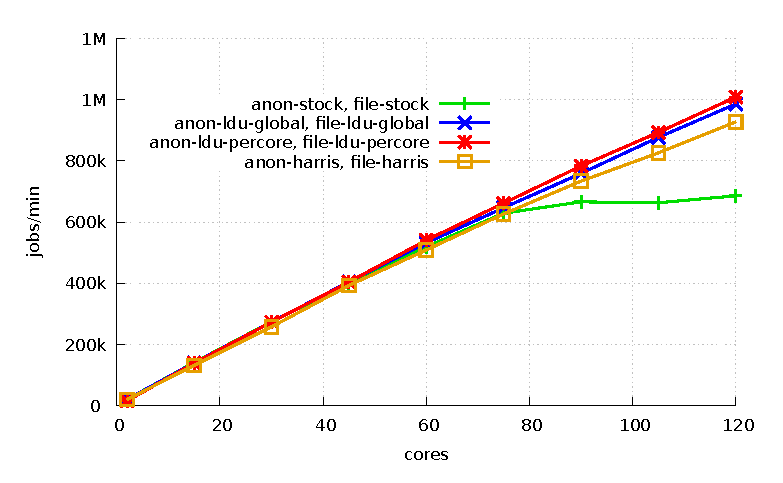
\includegraphics[scale=1]{graph/aim7.eps}
  \end{center}
  \caption{AIM7-multiuser 확장성.}
  \label{fig:aim7}
\end{figure}

\begin{figure*}[tb]
    \centering
    \begin{subfigure}[b]{1\textwidth}
  \begin{center}
        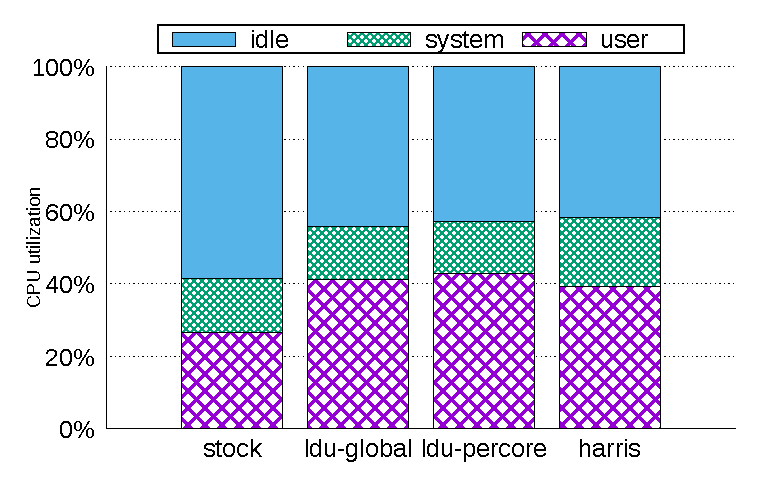
\includegraphics[scale=0.7]{graph/aim7_cpuutils.eps}
  \end{center}
    \end{subfigure}%
    \centering
    \caption{120코어에서 AIM7 CPU 사용량.}
    \label{fig:utilization_aim7}
    
\end{figure*}

\begin{figure*}[tb]
    \centering
    \begin{subfigure}[b]{1\textwidth}
  \begin{center}
        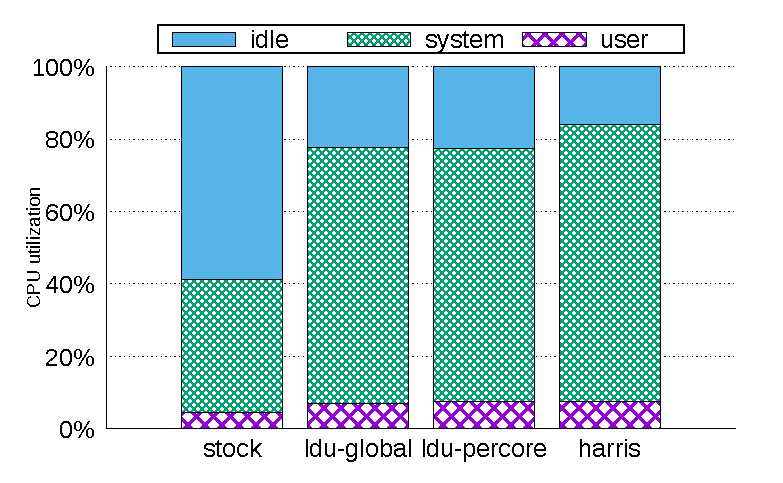
\includegraphics[scale=0.7]{graph/exim_cpuutils.eps}
  \end{center}
    \end{subfigure}
    \centering
    \caption{120코어에서 EXIM CPU 사용량. }
    \label{fig:utilization_exim}
    
\end{figure*}

\begin{figure*}[tb]
    \centering
    \begin{subfigure}[b]{1\textwidth}
  \begin{center}
        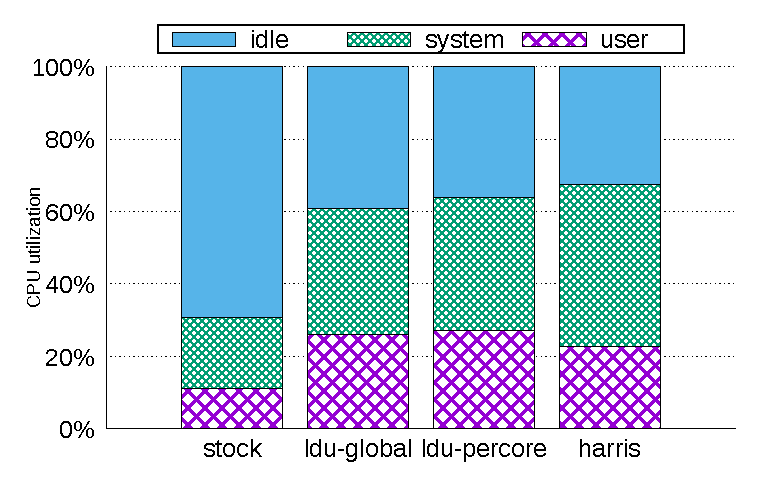
\includegraphics[scale=0.7]{graph/lmbench_cpuutils.eps}
  \end{center}
    \end{subfigure}
        \centering
    \caption{120코어에서 Lmbench CPU 사용량.}
    \label{fig:utilization_lmbench}
    
\end{figure*}

%$$$$$$$$$$$$$$$$$$$$$$$$$$$$$$$$$$$$$$$$$$$$$$$$$$$$$$$$$$$$$$$$$$$$$$$$$$$$$$$$
%Paragraph 1: AIM7 실험 결과
%$$$$$$$$$$$$$$$$$$$$$$$$$$$$$$$$$$$$$$$$$$$$$$$$$$$$$$$$$$$$$$$$$$$$$$$$$$$$$$$$


%$$$$$$$$$$$$$$$$$$$$$$$$$$$$$$$$$$$$$$$$$$$$$$$$$$$$$$$$$$$$$$$$$$$$$$$$$$$$$$$$
%Paragraph 1: 워크로드에 대한 설명
%$$$$$$$$$$$$$$$$$$$$$$$$$$$$$$$$$$$$$$$$$$$$$$$$$$$$$$$$$$$$$$$$$$$$$$$$$$$$$$$$
우리는 AIM7-multiuser를 사용하였다. 
이것은 AIM7의 워크로드 중 리눅스 \code{fork}에 집중된 벤치마크이다. 
이러한 multiuser 워크로드는 동시에 많은 프로세스를 생성 한 후 다양한 
일을 수행한다. 
또한 우리는 파일 시스템에 대한 병목현상을 줄이기 위해 리눅스 \code{tmpfs}를 사용하였고, 
코어 수에 비례하여 유져 수를 증가하였다.
 
%$$$$$$$$$$$$$$$$$$$$$$$$$$$$$$$$$$$$$$$$$$$$$$$$$$$$$$$$$$$$$$$$$$$$$$$$$$$$$$$$
%Paragraph 2: 실험 결과에 대한 설명
%$$$$$$$$$$$$$$$$$$$$$$$$$$$$$$$$$$$$$$$$$$$$$$$$$$$$$$$$$$$$$$$$$$$$$$$$$$$$$$$$
AIM7-multiuser에 대한 실험 결과는 그림 ~\ref{fig:aim7}과 같다.
75코어 전 까지는 수정 안한 리눅스는 확장성이 일정하나, 그 이후에는 직렬화된 업데이트 
연산 때문에 병목 현상이 생긴다. 
하지만 120코어까지 Harris 링크드 리스트와 우리의 LDU는 높은 확장성을 가진다.
그 이유는 워크로드들이 업데이트 연산과 읽기-쓰기 세마포어(\code{anon\_vma->rwsem},
\code{mapping->i\_mmap\_rwsem}) 없이 실행될 수 있기 때문이다.
LDU의 퍼코어 큐 버전은 가장 좋은 성능을 보여주고, 확장성도 뛰어나며, 
수정 안 한 리눅스에 비해 1.5배 빠르고 Harris 링크드 리스트보다 1.1배 빠르다.

게다가, 비록 LDU의 전역 큐 버전은 전역 CAS 명령어를 이용하여, 실행되지만, 이 
방법 역시 높은 성능과 확장성을 가진다.
그 이유는 LDU의 최적화 방법 때문에 전역 CAS에 대한 접근이 완화되기 때문이다.
이것은 120코어에서 퍼코어 버전에 비해 2\% 성능 저하가 생긴다. 
더욱이, 수정 안 한 리눅스는 가장 높은 유휴(IDLE) 시간(56\%)을 가진다(그림 ~\ref{fig:utilization_aim7}). 
그 이유는 2가지 세마포어(i.e.,
\code{anon\_vma->rwsem}, \code{mapping->i\_mmap\_rwsem}))를 얻기 위해 스레드가 블락에
걸리기 때문이다.
LDU가 Harris 커널 버전보다 높은 유휴시간을 가지지만, 처리량은 Harris 방법보다 더 높다.
이것은 우리의 LDU 알고리즘이 효율적이라는 것을 보여준다. 

\begin{figure}[tb]
  \begin{center}
    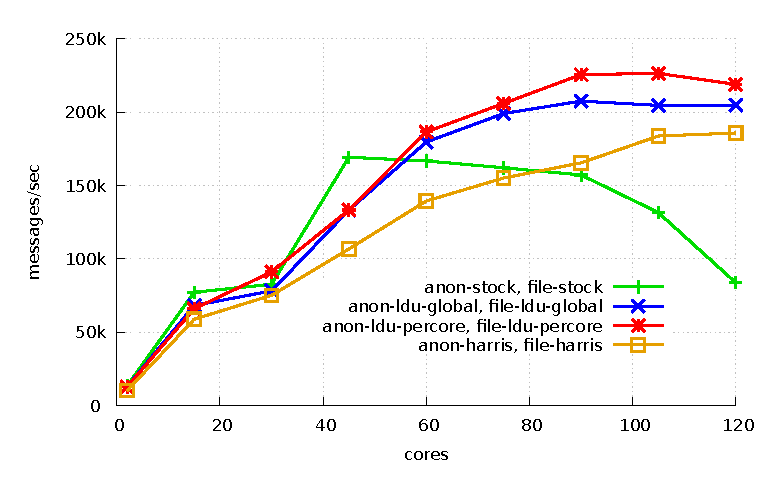
\includegraphics[scale=1]{graph/exim.eps}
  \end{center}
  \caption{Exim 확장성.}
  \label{fig:exim}
\end{figure}

\subsection{Exim}
%$$$$$$$$$$$$$$$$$$$$$$$$$$$$$$$$$$$$$$$$$$$$$$$$$$$$$$$$$$$$$$$$$$$$$$$$$$$$$$$$
%Paragraph 1:  EXIM 실험 결과
%$$$$$$$$$$$$$$$$$$$$$$$$$$$$$$$$$$$$$$$$$$$$$$$$$$$$$$$$$$$$$$$$$$$$$$$$$$$$$$$$

\begin{figure}[tb]
  \begin{center}
    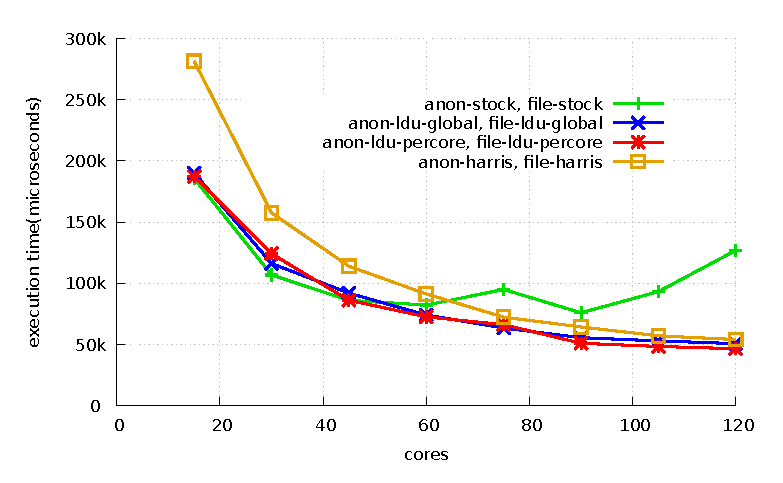
\includegraphics[scale=1]{graph/lmbench.eps}
  \end{center}
  \caption{Lmbench의 프로세스 관리 벤치마크에 대한 실행시간.}
  \label{fig:MicroBench}
\end{figure}

%$$$$$$$$$$$$$$$$$$$$$$$$$$$$$$$$$$$$$$$$$$$$$$$$$$$$$$$$$$$$$$$$$$$$$$$$$$$$$$$$
%Paragraph 1: 워크로드에 대한 설명
%$$$$$$$$$$$$$$$$$$$$$$$$$$$$$$$$$$$$$$$$$$$$$$$$$$$$$$$$$$$$$$$$$$$$$$$$$$$$$$$$
Exim의 성능에 대한 확장성을 측정하기 위하여, 우리는 매니코어 확장성 벤치마크 중 하나인 MOSBENCH를 이용하였다. 
본래 이메일(E-mail) 서버인 Exim의 디자인은 확장성이 있게 설계되었다. 
그 이유는 Exim의 메시지 전달자는 리눅스의 프로세스 기반으로 동작하며, 
여러 프로세스가 병렬적인 방법을 사용하여 메시지를 메일 박스에 전달한다.
이러한 Exim은 \code{fork}가 많이 발생하는 워크로드 중 하나이다. 
클라이언트를 같은 장치에서 실행하였고, 
각각의 클라인언트는 메일 파일에 대한 충돌을 막기 위해, 메시지를 여러 유저에게 보낸다.
Exim은 파일 시스템에서 병목 현상이 발생된다~\cite{SilasBoydWickizer2010LinuxScales48}.
그 이유는 메시지의 바디가 각각의 유저 메일 파일에 추가되기 때문이다.
따라서 우리는 파일 시스템의 병목 지점을 제거하기 위해 분활 된 \textit{tmpfs}를 사용하였다. 

%$$$$$$$$$$$$$$$$$$$$$$$$$$$$$$$$$$$$$$$$$$$$$$$$$$$$$$$$$$$$$$$$$$$$$$$$$$$$$$$$
%Paragraph 2:실험 결과에 대한 설명
%$$$$$$$$$$$$$$$$$$$$$$$$$$$$$$$$$$$$$$$$$$$$$$$$$$$$$$$$$$$$$$$$$$$$$$$$$$$$$$$$
그림~\ref{fig:exim}과 같이 Exim의 결과는 수정안 한 리눅스 커널은 
60코어까지 확장성이 좋게 동작을 한다. 
하지만 60코어 근처부터 확장성이 떨어지는 모습을 볼 수 있다.
45코어 지점에서는 수정 안한 리눅스 커널의 성능이 높게 나오는데, 이것은 LDU의 방법이 
궁극적으로 업데이트 연산을 뒤로 미루는 방법이기 때문에, 락 경합이 덜 발생하면, 오히려 로깅하는 오버헤드 때문에 
성능이 떨어질 수 있다. 
이것은 LDU가 여전히 특정 워크로드와 함께 적은 코어에서의 문제점을 가지고 있다는 것을 보여준다.
하지만 60코어 이후에는 성능이 역전 되어 좋은 성능을 보인다. 

Harris와 LDU는 105코어까지 높은 성능 확장성을 보인다. 
그 이유는 이 두 방법은 세마포어 때문에 기다리는 현상 없이 동시에 업데이트 연산이 가능하기 때문이다. 
LDU의 퍼코어 큐 버전은 더 좋은 성능을 가진다.
그 이유는 이것은 캐시 일관성과 관련한 오버헤드가 없기 때문이며, 120코어에서 수정 안한 
리눅스보다 2.6배 성능 향상을 가지며, Harris 보다 1.2배의 성능 향상을 가진다.
비록 확장성 있는 기술을 적용하였지만, Exim은 105코어부터 성능 확장성에 대해서 문제가 생긴다.
그 이유는 Exim 프로세스들은 상대적으로 큰 크기의 가상 메모리를 사용하기 때문이다.
이것은 결국 프로세스가 종료될 때 가상 메모리에 대한 초기화 오버헤드를 낳으며,
결국 많은 소프트 페이지 폴트(Soft Page Fault)를 야기한다. 
이것은 특히 NUMA 구조와 같은 구조에서는 원격 메모리를 접근하는 현상 때문에 더욱 많은 오버헤드를 야기한다. 
Harris 링크드 리스트는 15\%의 유휴 시간을 가진 반면, 퍼코어 큐 버전의 LDU는 22\%의 유휴 시간을 가진다.
그 이유는 LDU의 효율적인 알고리즘 때문이다(그림~\ref{fig:utilization_exim}).

\subsection{Lmbench}
%$$$$$$$$$$$$$$$$$$$$$$$$$$$$$$$$$$$$$$$$$$$$$$$$$$$$$$$$$$$$$$$$$$$$$$$$$$$$$$$$
%Paragraph 1: %워크로드에 대한 설명
%$$$$$$$$$$$$$$$$$$$$$$$$$$$$$$$$$$$$$$$$$$$$$$$$$$$$$$$$$$$$$$$$$$$$$$$$$$$$$$$$
Lmbench는 다양한 마이크로(Micro) 벤치마크를 포함하고 있다. 
우리는 이러한 다양한 마이크로 벤치마크 중 프로세스 관리에 대한 워크로드를 사용하였다. 
워크로드는 기본적인 프로세스 관리에 대한 프로세스 생성, 
프로그램 시작, 그리고 문맥교환들에 대해서 성능을 측정한다.
그리고 우리는 프로세스 생성에 대한 워크로드에 대해 병렬 옵션 값인 1000을 사용하여 수행하였다. 

%$$$$$$$$$$$$$$$$$$$$$$$$$$$$$$$$$$$$$$$$$$$$$$$$$$$$$$$$$$$$$$$$$$$$$$$$$$$$$$$$
%Paragraph 2: 실험 결과에 대한 설명
%$$$$$$$$$$$$$$$$$$$$$$$$$$$$$$$$$$$$$$$$$$$$$$$$$$$$$$$$$$$$$$$$$$$$$$$$$$$$$$$$
Lmbench의 결과는 그림~\ref{fig:MicroBench}에서 보여주며, 세로축에 대한 결과는 실행 시간이다.
45코어까지, 수정 안 한 리눅스 커널은 일정한 확장성을 보이며, 그 이후 실행시간을 늘어난다.
퍼코어 버전의 LDU는 120코어에서 수정 안 한 리눅스 커널에 2.7배 성능향상으로 보이며, 
Harris 리스트에 비해 1.1배의 성능향상을 보인다.
수정 안 한 리눅스는 69\%의 유휴 시간을 가진 반면 다른 방법들은 약 35\% 정도의 유휴시간을 가진다.
그 이유는 수정 안한 리눅스 커널은 2가지 RMAP 세마포어(\code{anon\_vma->rwsem},
\code{mapping->i\_mmap\_rwsem})(그림~\ref{fig:utilization_lmbench})를 기다리기 때문이다. 
사실, 우리의 LDU의 개발 동기는 120코어에서 성능과 확장성을 개선하는 것이다. 
따라서 우리는 적은 코어(30코어 이내)에서의 성능은 고려하지 않았다.
하지만 30코어까지 우리의 LDU는 수정 안한 리눅스 커널과 비슷한 성능을 보인다. 
반면, Harris 링크드 리스트는 60코어 까지 안 좋은 성능을 보여준다. 
이러한 현상은 LDU가 효율적인 알고리즘 이라는 것을 보여준다.

\subsection{업데이트 비율}

%$$$$$$$$$$$$$$$$$$$$$$$$$$$$$$$$$$$$$$$$$$$$$$$$$$$$$$$$$$$$$$$$$$$$$$$$$$$$$$$$
%Paragraph 2:  실험을 수행한 이유
%$$$$$$$$$$$$$$$$$$$$$$$$$$$$$$$$$$$$$$$$$$$$$$$$$$$$$$$$$$$$$$$$$$$$$$$$$$$$$$$$
본 논문에서 제안하는 LDU는 Update-heavy한 자료구조를 위한 방법이다. 
따라서 리더가 많아질 경우 성능이 떨어지는 단점을 가진다. 
그 이유는 LDU의 읽기 연산은 로그를 적용하는 \code{synchronize} 함수를 호출하므로, 
그 동안 쌓인 로그들을 적용하게 되는데, \code{synchronize} 함수의 
연산 때문에 읽기 연산이 많이 지면 성능이 떨어진다.
따라서, 우리는 어느정도 까지 영향을 미치는지 확인하기 위해, 연산이 자주 발생하는 경우를 
대상으로 실험을 하였다. 

읽기 연산에 대한 효과를 이해하기 위해, 읽기 연산을 업데이트 연산의 비율에 
맞게 추가하여 성능을 측정하는 실험을 하였다.
실험을 단순화 하기 위해 익명 RMAP 자료 구조는 LDU의 전역 큐 버전을 이용하였고, 
파일 RMAP에 대해서는 순차적으로 읽기 연산(\code{lock}, \code{synchronize}) 비율을 증가 시켰다.
예를 들어 99\%는 파일 RMAP에 대해서 업데이트 연산이 99번 수행할 때 1번의 읽기 연산이 
일어나는 것을 의미하고, 순차적으로 90\%는 9번 업데이트에 1번의 읽기 연산을 의미한다.

\begin{figure}[h!]
    \centering
    \begin{subfigure}[b]{1\textwidth}
        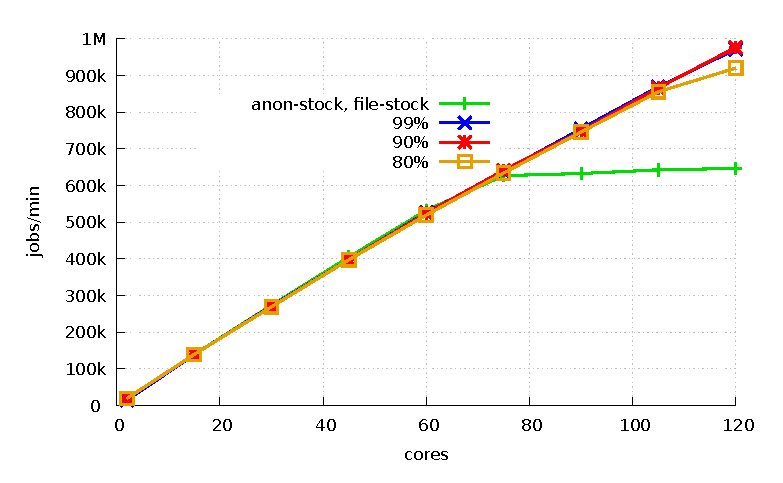
\includegraphics[height=2.5in]{graph/ratio_aim7_core.eps}
    \end{subfigure}%
    \caption{업데이트 비율에 따른 AIM7 확장성.}
    \label{fig:UpdateRate_aim7_2}
\end{figure}
 
 
%$$$$$$$$$$$$$$$$$$$$$$$$$$$$$$$$$$$$$$$$$$$$$$$$$$$$$$$$$$$$$$$$$$$$$$$$$$$$$$$$
%Paragraph 2: 실험 결과에 대한 설명
%$$$$$$$$$$$$$$$$$$$$$$$$$$$$$$$$$$$$$$$$$$$$$$$$$$$$$$$$$$$$$$$$$$$$$$$$$$$$$$$$
그림~\ref{fig:UpdateRate_aim7_2}는 AIM7의 실험 결과를 보여준다.
AIM7의 경우 다른 2가지 벤치마크(Exim, Lmbench)에 비해 덜 \code{fork}에 의존적인 
벤치마크이기 때문에, 읽기 연산이 호출되는 간격이 상대적으로 짧다.
그 결과, 비록 자료구조가 80\%의 업데이트 비율(4개의 업데이트 연산 일때 1개의 읽기 연산을 수행)을 
가지더라도, 수정 안 한 리눅스에 비해 높은 성능을 가진다. 
AIM7의 성능에 대한 확장성은 90\% 이상의 경우 경우 높은 성능 확장성을 가진다.
 
\begin{figure}[h!]
    \centering
    \begin{subfigure}[b]{1\textwidth}
        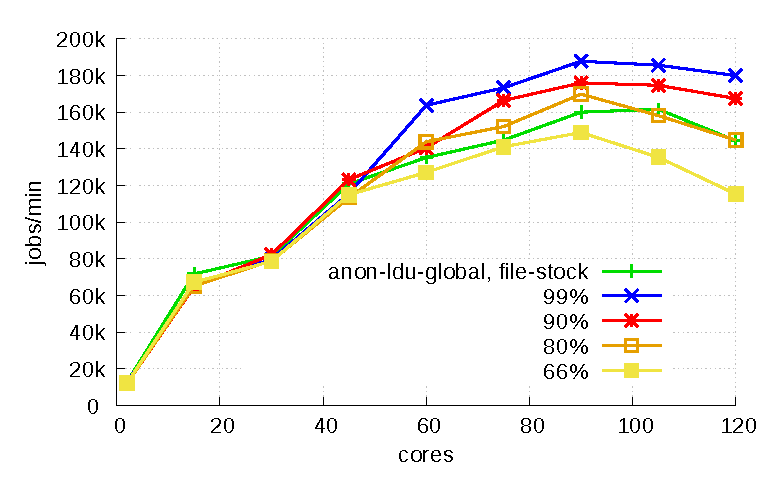
\includegraphics[height=2.5in]{graph/ratio_exim_core.eps}
    \end{subfigure}%
    \caption{업데이트 비율에 따른 Exim 확장성.}
    \label{fig:UpdateRate_exim_2}
\end{figure}


%$$$$$$$$$$$$$$$$$$$$$$$$$$$$$$$$$$$$$$$$$$$$$$$$$$$$$$$$$$$$$$$$$$$$$$$$$$$$$$$$
%Paragraph 2: 실험 결과에 대한 설명
%$$$$$$$$$$$$$$$$$$$$$$$$$$$$$$$$$$$$$$$$$$$$$$$$$$$$$$$$$$$$$$$$$$$$$$$$$$$$$$$$
Exim은 \code{fork}를 많이 호출하는 워크로드 중 하나이다. 
따라서 업데이트 연산이 빨리 호출되는 특징을 가지며, 이것은 읽기 연산의 간격도 짧다는 것을 의미한다.
즉 AIM7과는 다르게 \code{synchronize} 함수가 자주 호출된다는 것을 의미한다.
그 결과, 80\% 이하의 업데이트 연산 비율을 가지면 수정 안 한 리눅스 보다 안 좋은 성능을 가진다.
LDU는 90\% 이상의 업데이트 가질 때 부터 더 높은 성능을 가진다.

\begin{figure}[h!]
    \centering
    \begin{subfigure}[b]{1\textwidth}
        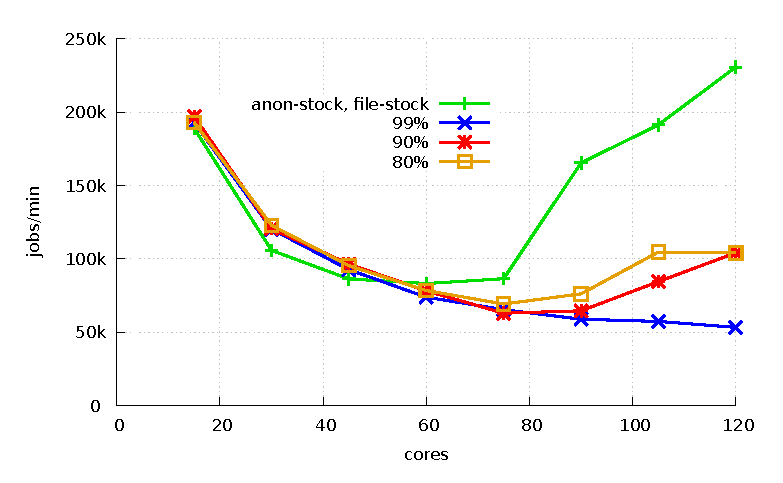
\includegraphics[height=2.5in]{graph/ratio_lmbench_core.eps}
    \end{subfigure}%
    \caption{업데이트 비율에 따른 Lmbench 확장성.}
    \label{fig:UpdateRate_lmbench_2}
\end{figure}

%$$$$$$$$$$$$$$$$$$$$$$$$$$$$$$$$$$$$$$$$$$$$$$$$$$$$$$$$$$$$$$$$$$$$$$$$$$$$$$$$
%Paragraph 2: 실험 결과에 대한 설명
%$$$$$$$$$$$$$$$$$$$$$$$$$$$$$$$$$$$$$$$$$$$$$$$$$$$$$$$$$$$$$$$$$$$$$$$$$$$$$$$$
Lmbench는 Exim과 비슷하게 \code{fork}가 자주 호출 되는 워크로드이다.
Lmbench는 실행 시간을 보여주므로, 낮을 수록 높은 성능을 보여준다. 
실험 결과 Exim과 비슷한 결과를 보이는데, 이것은 수정 안 한 리눅스가 80\%의 업데이트 
비율을 가질 때 더 좋은 성능을 가진다.
하지만 Lmbench는 굉장히 \code{fork}가 자주 호출되는 마이크로 벤치마크이기 때문에 업데이트 연산의 비율이 
90\%가 되면 수정 안한 리눅스 보다는 성능이 좋지만, 확장성이 떨어지는 특징을 가진다.
하지만 LDU는 읽기가 상당히 자주 호출되는 워크로드라도 업데이트 비율이 90\% 이상이면 
높은 성능을 보여준다.
 
